
%\documentclass[review]{elsarticle}
\documentclass[12pt]{article}

\usepackage{lineno}

\usepackage{amsmath}
\usepackage{amsfonts}
\usepackage{amsthm}
\usepackage{graphicx}
\usepackage{natbib}
\usepackage{setspace}
\doublespacing
%\usepackage{url}
\usepackage{subfig}
\DeclareMathOperator*{\argmin}{argmin}
\newcommand*{\argminl}{\argmin\limits}
\newtheorem{prop}{Proposition}
\newtheorem{corollary}{Corollary}

%\modulolinenumbers[5]

%\journal{Statistics and Probability Letters}

%%%%%%%%%%%%%%%%%%%%%%%
%% Elsevier bibliography styles
%%%%%%%%%%%%%%%%%%%%%%%
%% To change the style, put a % in front of the second line of the current style and
%% remove the % from the second line of the style you would like to use.
%%%%%%%%%%%%%%%%%%%%%%% %% Numbered %\bibliographystyle{model1-num-names} %% Numbered without titles %\bibliographystyle{model1a-num-names} 
%% Harvard
%\bibliographystyle{model2-names.bst}\biboptions{authoryear}

%% Vancouver numbered
%\usepackage{numcompress}\bibliographystyle{model3-num-names}

%% Vancouver name/year
%\usepackage{numcompress}\bibliographystyle{model4-names}\biboptions{authoryear}

%% APA style
%\bibliographystyle{model5-names}\biboptions{authoryear}

%% AMA style
%\usepackage{numcompress}\bibliographystyle{model6-num-names}

%% `Elsevier LaTeX' style
%\bibliographystyle{elsarticle-num}
\bibliographystyle{plain}
%%%%%%%%%%%%%%%%%%%%%%%

\begin{document}

%\begin{frontmatter}

\title{Clinical Trial Design Using A Stopped Negative Binomial Distribution}
\maketitle
%\tnotetext[mytitlenote]{This research was supported by grants R01CA131301, 
%R01CA157749, R01CA148996, R01CA168733, and PC50CA196530 awarded by the 
%National Cancer Institute along with support from the Yale Comprehensive Cancer 
%Center and the Yale Center for Outcomes Research. We would also like 
%to thank Rick Landin at Ignyta Inc. for his suggestions.}

%% Group authors per affiliation:
%\author{Elsevier\fnref{myfootnote}}
%\address{Radarweg 29, Amsterdam}
%\fntext[myfootnote]{Since 1880.}

%% or include affiliations in footnotes:
%\author{Michelle DeVeaux}
%\ead{michelle.deveaux@yale.edu}

%\author{Michael J. Kane$^*$\footnote{* Corresponding author}}
%\ead{michael.kane@yale.edu}

%\author{Daniel Zelterman}
%\ead{daniel.zelterman@yale.edu}

%\address{Department of Biostatistics\\ School of Epidemiology and Public Health\\ Yale University, New Haven, CT}

\begin{abstract}
We introduce a discrete distribution suggested by curtailed
sampling rules common in early-stage clinical trials. We derive the
distribution of the smallest number of independent and identically
distributed Bernoulli trials needed to observe either $s$ successes 
or $t$ failures. This report provides a closed-form expression for the 
mass function and illustrates limiting approximations.
\end{abstract}

%\begin{keyword}
%discrete distribution\sep curtailed sampling
%\end{keyword}

%\end{frontmatter}

%\linenumbers

\section{Introduction and Motivation}

Consider a prototypical early phase, single-arm clinical trial in which 
17 patients
are enrolled and treated. Suppose the Bernoulli probability of a patient 
responding to treatment is $p=0.2$ 
under the null hypothesis that the treatment is not effective.
If seven or more patients out of these 17 respond to the treatment then we 
reject this hypothesis and the treatment is deemed successful at 
a significance level of $0.1$.  If fewer than seven respond then the null 
hypothesis is not 
rejected and the treatment is deemed ineffective. The trial is 
realized as a sequence of Bernoulli($p$) samples stopping when either
the specified number of responders or non-responders is reached.

If all 17 patients are enrolled at once, as in the classic
design, then the sample size is 17. However, in most clinical trials the
patients are enrolled sequentially over time.
In the present example, observing seven
successful patients ends the trial and so the number of enrollees required
could be as small as seven. Similarly 11
observed treatment failures also ends the trial. This sampling mechanism, in
which the experiment ends as soon as any predefined endpoint is reached, is
called {\em curtailed sampling}. Under curtailed sampling, the range of the
sample size for this trial is seven through 17.

\begin{figure}[bp!]
\centering
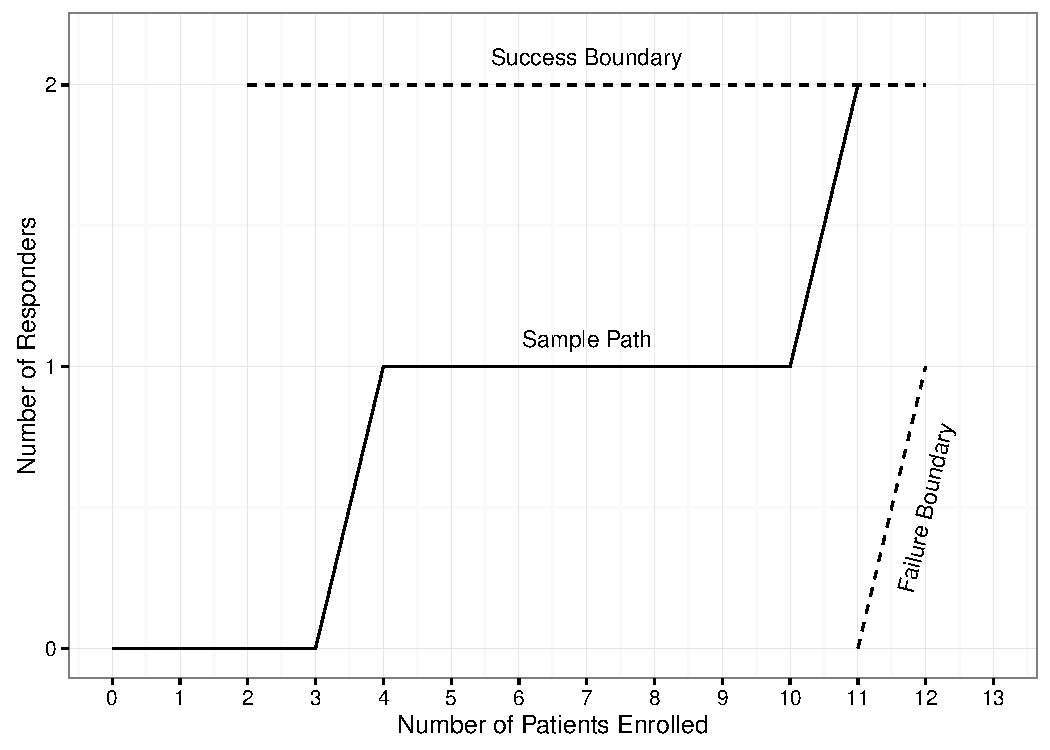
\includegraphics[width=\textwidth]{KanePlot.pdf}
\caption{
A hypothetical realization of the trial.
}
\label{fig:kane_viz}
\end{figure}

A hypothetical sample path is illustrated in Fig.~\ref{fig:kane_viz}.
The vertical axis denotes the number of
successful outcomes. The horizontal axis counts the number of patients 
enrolled. The horizontal and tilted vertical boundaries represent
endpoints for the trial. In this case, a seventh response was reached on
the $15^{\text{th}}$ enrollment.
Since the success boundary is reached, we say the treatment succeeds.

%\begin{figure}[bp!]
%\centering
%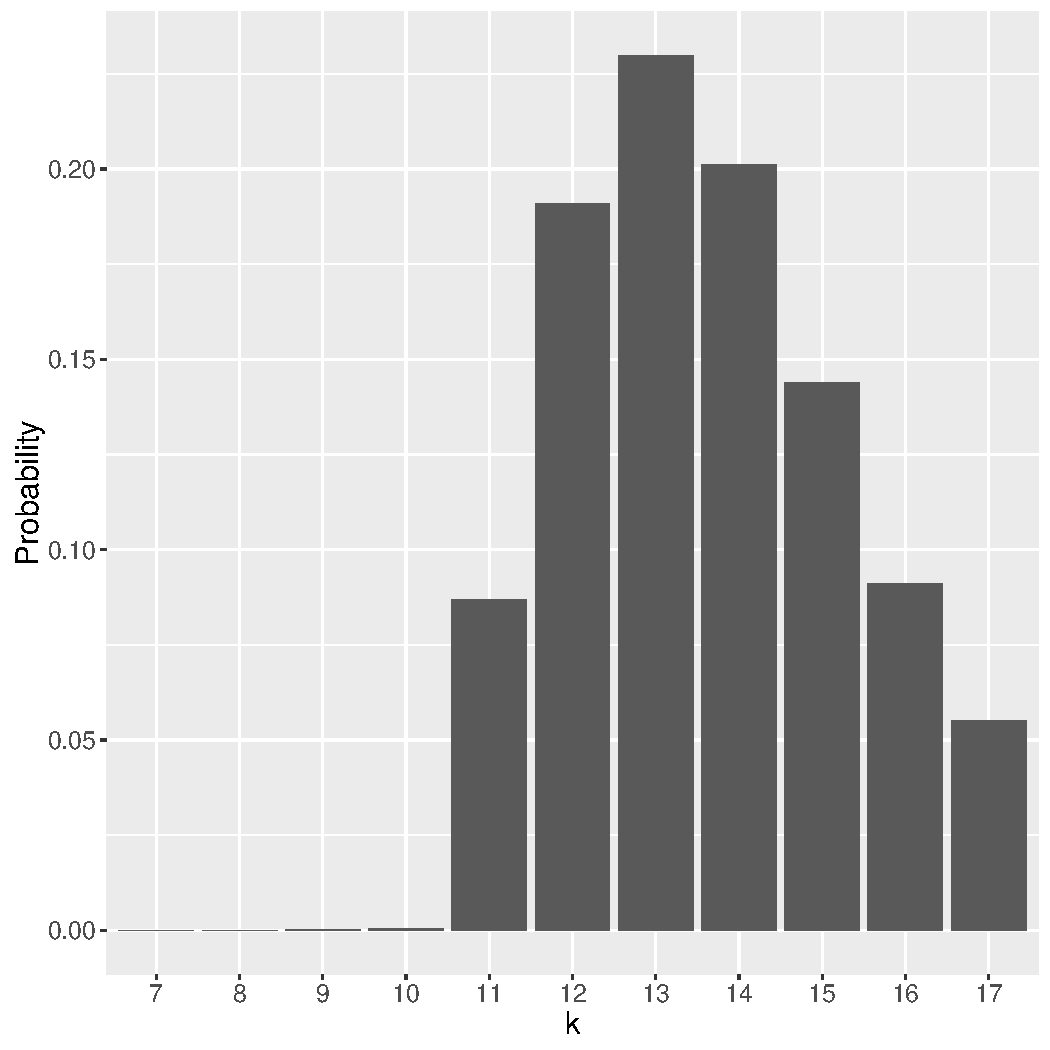
\includegraphics[width=\textwidth]{snb-first-plot.pdf}
%\caption{
%The probability mass function for a trial where $p$ 
%is 0.045 and where the trial stops
%after two patients respond or 11 patients do not respond.
%}
%\label{fig:first-plot}
%\end{figure}

\begin{figure}[bp!]
\centering
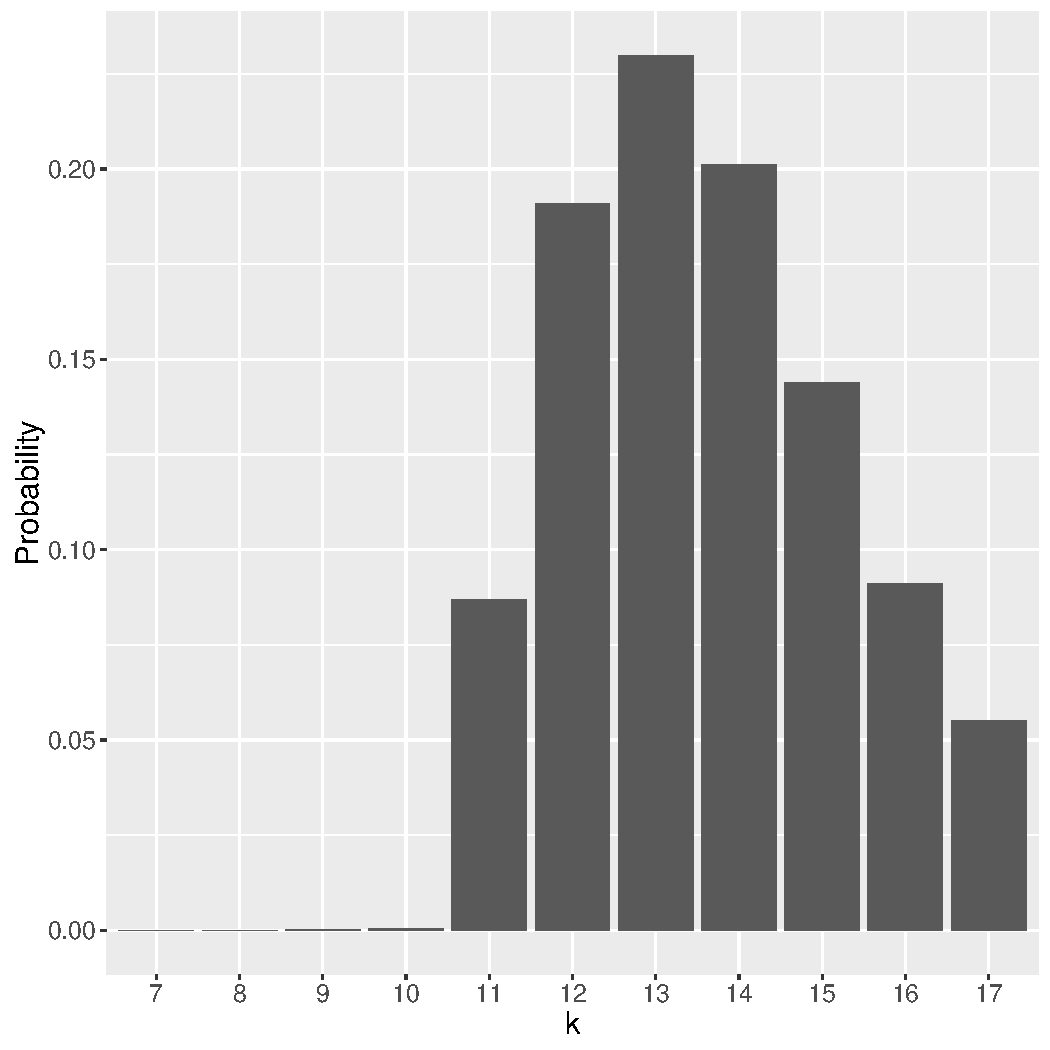
\includegraphics[width=\textwidth]{snb-first-plot.pdf}
\caption{
The distribution of the sample size in a trial that stops after seven patients
respond to treatment or 11 do not when $p=0.2$.
}
\label{fig:kane_viz}
\end{figure}

\begin{figure}[bp!]
\centering
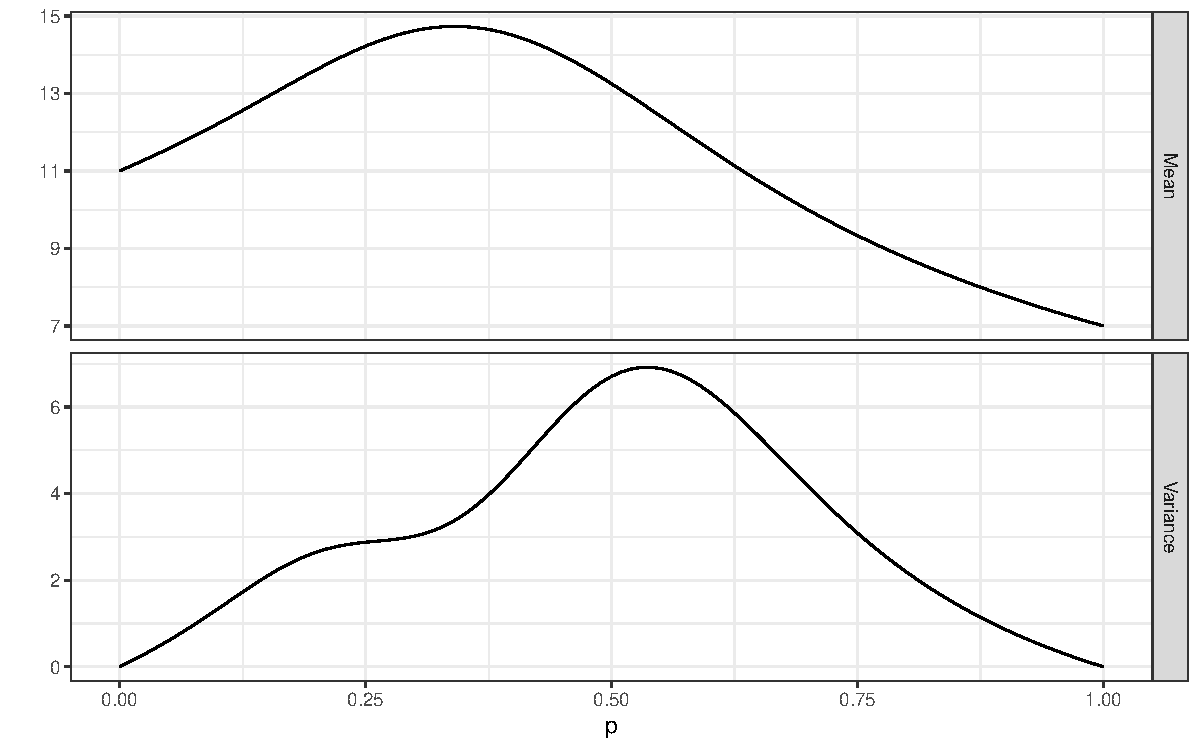
\includegraphics[width=\textwidth]{mean-and-variance.pdf}
\caption{
The effect of varying $p$ between zero and one when the trial stops after
seven patients respond or 11 do not.
}
\label{fig:kane_viz}
\end{figure}


%\begin{figure}[bp!]
%\centering
%\subfloat[enrollment distribution]{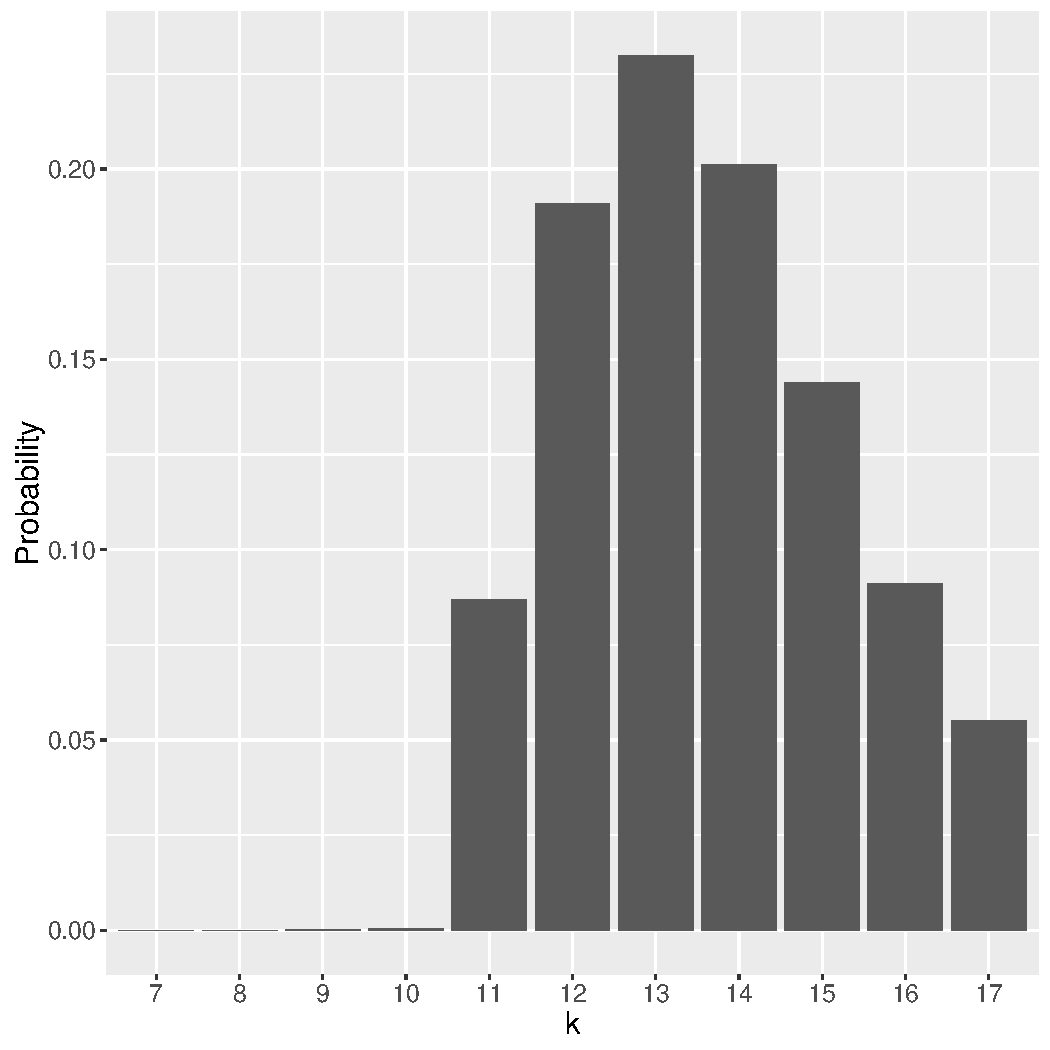
\includegraphics[width=0.45\textwidth]{snb-first-plot.pdf}}
%\hfill
%\subfloat[mean and variance varying $p$]{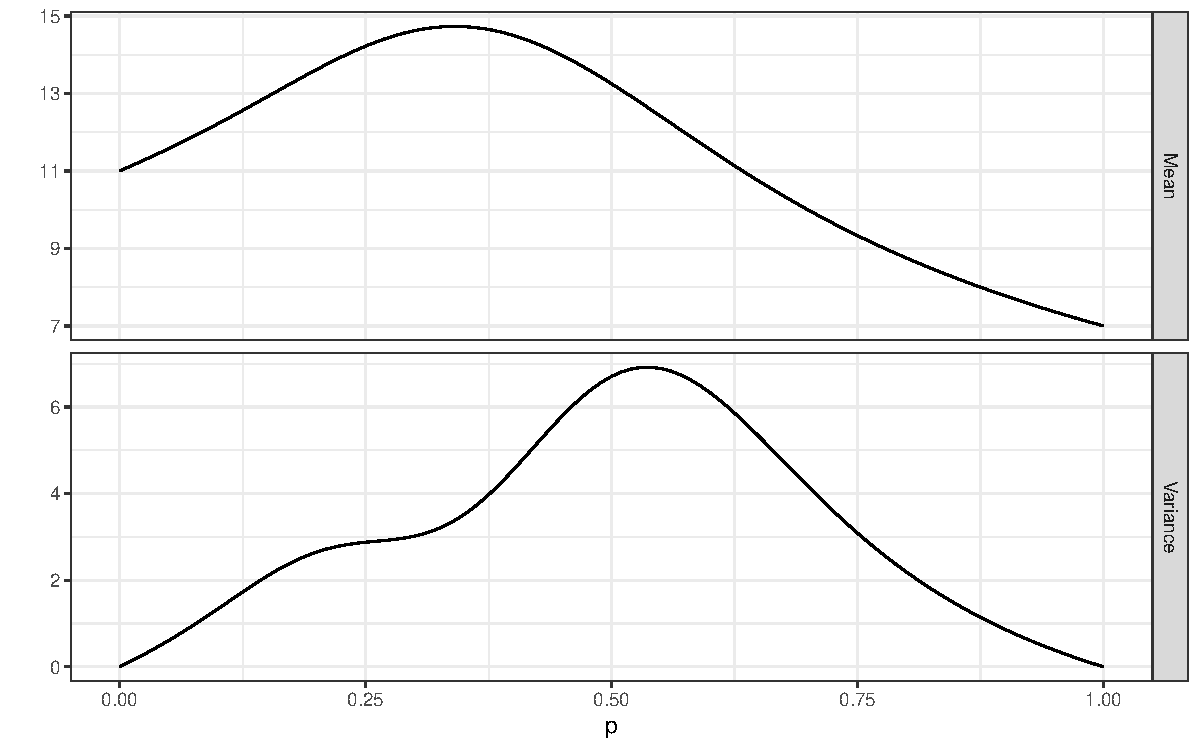
\includegraphics[width=0.45\textwidth]{mean-and-variance.pdf}}
%\caption{
%The distribution of the sample size in a trial that stops after seven 
%patients respond to treatment
%or 11 patients do not. Panel (a) shows the distribution when
%$p = 0.2$. The mean and variance of the distribution varying $p$ 
%between zero and one are shown in panel (b).
%}
%\label{fig:exp-and-var}
%\end{figure}

The distribution of the number of trial enrollments is shown in 
Fig.~\ref{fig:kane_viz}. There is relatively little probability mass
for values of sample size equal to seven through 10 since $p$ is small and it 
is unlikely the treatment will succeed quickly.
%The probability mass is concentrated at the 
%$11^{\text{th}}$ and $12^{\text{th}}$ step since $p$ 
%is small and for most realizations reach 11 
%non-responders before reaching 2 responders.
Fig.~\ref{fig:kane_viz} shows the expected value and variance for the
number of trial enrollments varying $p$ between zero and one. When $p$ is
small then the treatment
is more likely to fail shortly after the $11^{\text{th}}$ enrollment.
When $p$ is large then the treatment is more likely to succeed and the 
number of enrollees approaches seven from above. 

When $p=0$ or $1$ the processes are deterministic and variance is zero.
Values between zero and one change the mixing proportions of 
the two endpoints. The saddle around $p=0.25$ results from inequality 
in the size of the support of the two endpoints.

%\begin{table}[t!]
%\caption{Characteristics of the Stopped Negative Binomial Distribution}
%\label{tab:snb}
%\begin{center}
%\begin{tabular}{|c|l|} \hline
%Parameters & $p$ the success probability ($0\leq p \leq 1$; $q = 1-p$) \\
%           & $s$ the number of successes before stopping ($s=1, 2, ...$)\\
%           & $t$ the number of failures before stopping ($t=1, 2, ...$)\\ \hline
%Support & min$(s,t) \leq k \leq s+t-1$  \\ \hline
%$\mathbb{P}[Y=k]$ & ${k-1 \choose s-1} p^s (1-p)^{k-s} I_{\{s \leq k \leq s+t-1\}\}}+ {k-1 \choose t-1} (1-p)^s p^{k-t} I_{\{t \leq k \leq s+t-1\}}$\\ \hline
%$\mathbb{P}[Y \leq k]$ & $2 - \mathcal{I}_{q}(k+1, s) - \mathcal{I}_{p}(k+1, t)$\\ 
%    & where $\mathcal{I}$ is the regularized incomplete beta function.\\ \hline
%Mean & $\frac{s}{p} \mathcal{I}_p(s,t) + \frac{p^{s-1} q^{t-1}}{B(s,t)} +
%  \frac{t}{q} \mathcal{I}_q(t,s) + \frac{p^{t-1} q^{s-1}}{B(s,t)}$\\ 
%  & where $B$ is the beta function \\ \hline
%MGF & $\left(\frac{p e^x}{1 - qe^x}\right)^s 
%  \mathcal{I}_{1-qe^x} (s, t) + \left(\frac{qe^x}{1-pe^x}\right)^t 
%  \mathcal{I}_{1-pe^x}(t, s) $\\ \hline
%Predictive Distribution & 
%${k-1 \choose s-1} \frac{B\left(\alpha+s, k-s+\beta \right)}{B(\alpha, \beta)}+
%{k-1 \choose t-1} \frac{B\left(\alpha + k-t, t+\beta\right)}{B(\alpha,\beta)}$\\
%& for $p$ distributed as Beta($\alpha$, $\beta$). \\ \hline
%\end{tabular}
%\end{center}
%\end{table}

In the rest of this work, we derive the distribution of the number of 
enrollees needed
to observe either $s$ successes or $t$ failures. We refer to this distribution
as the Stopped Negative Binomial (SNB). 
%Some of its characteristics are summarized in Tab.~\ref{tab:snb}.
This paper derives this distribution and explores its properties.
%The next section introduces our notation and basic results
%including the density of the distribution along with a description of
%its relation to other distributions. 
Section 2 derives the distribution function
based on a defined Bernoulli process and gives some basic properties.
Section 3 shows how the distribution is related to other standard
distributions and connects the SNB tail probability to the binomial tail 
probability.
Section 4 derives the moment generating function.
Section 5 derives the predictive and posterior distributions when $p$ has a 
beta prior distribution.

\section{Probability Mass Function}
\label{notation.section}

Let $\,b_1, b_2, \ldots \,$ denote a sequence of independent, identically
distributed, Bernoulli random variables with $\mathbb{P}[b_i=1]=p$ and
$\mathbb{P}[b_i = 0] = 1-p$, for
probability parameter $0\leq p \leq 1$. In the clinical trial setting
$\,b_i = 1$ corresponds to a patient responding to treatment.  

Let $s$ and $t$ be positive integers.  Define the SNB random
variable $Y$ as the smallest
integer value such that $\,\{b_1, \ldots , b_Y\}\,$ contains {\em either}
$\,s\,$ responders {\em or} $\,t\,$ non-responders. That is, the SNB 
distribution of $Y$ is the smallest integer such that either
$\sum_i^Y b_i = s$ or $\sum_i^Y 1-b_i = t$.

The distribution of $\,Y\,$ has support on integer values in the range
\begin{equation*}               
     \min(s,t) \leq \; Y \;\leq s+t-1  \label{range.y.eq}.
\end{equation*}
The probability mass function is
\begin{equation} \label{eqn:pmf}
\mathbb{P} [Y=k] = S(k, p, s) \ I_{\{s \leq k \leq s+t-1\}} + 
  S(k, 1-p, t) \ I_{\{ t \leq k \leq s+t-1 \}}
\end{equation}
where $I_{\{f\}}$ is the {\em indicator function}, taking the value 
of one if $f$ is true and zero otherwise, and
\begin{equation} \label{eqn:N}
S(k, p, s) = {k-1 \choose s-1} p^s (1-p)^{k-s} 
\end{equation}
is the negative binomial probability mass. 
The CDF of the negative binomial is commonly expressed in terms of the
{\em regularized incomplete beta function} \citep{Olver2010}. Using standard
notation, (\ref{eqn:N}) is written as $\mathcal{I}_{1-p}(t, s)$.

To prove (\ref{eqn:pmf}), consider the
process $\mathbf{X} = \left\{X(k) : k = 0,1,... \right\}$
with $X(0)=0$ and
\begin{equation*} \label{eqn:proc}
X_{k+1} = X_k + b_{k+1} \ I_{\{ k-t < X_k < s\}}.
\end{equation*}
At each step a patient's outcome is measured. In Fig.~\ref{fig:kane_viz} 
we consider a graphical illustration of the plot $X_k$ against
$k$. If the outcome of the $k$th patient responds to treatment then the process 
advances diagonally in the positive horizontal and vertical direction. 
If the $k$th patient does not respond
then the sample path advances in the positive horizontal direction only. The
process continues until either $X_k = s$ or $X_k = k-t$ corresponding to the
success and failure boundaries in Fig. \ref{fig:kane_viz}, respectively.

\begin{prop}
The distribution of the stopping time
\begin{equation*}
Y = \argminl_k \left[X_k \geq s \cup X_k \leq k-t \right]
\end{equation*}
is given at (\ref{eqn:pmf}).
\end{prop}
\begin{proof}
%The proof will proceed in two parts. First, a combinatorial justification 
%will be given for the probability mass value on each element of the support. 
%Second, it will be shown that the sum of the masses over the support sums to 
%one.

The probability a given realization of $\mathbf{X}$ reaches $s$ at
the $k$th outcome is the probability that, at time $k-1$, there are $s-1$
successful outcomes and $k-s$ unsuccessful outcomes multiplied by
the probability of a final success at time $k$. This expression is given
in (\ref{eqn:N}). 
Similarly, the probability a given realization reaches $k-t$
is the probability that, at outcome $k-1$, there are $k-t$ successful outcomes
and $t-1$ unsuccessful outcomes multiplied by the probability of a final
unsuccessful outcome at time $k$. That is,
\begin{align*}
p {k-1 \choose s=1} p^{s-1} & (1-p)^{k-s} + (1-p) {k-1 \choose k-t} p^{k-t} (1-p)^{t-1} \\ 
& = S(k, p, s) + S(k, 1-p, t)
\end{align*}
as claimed in (\ref{eqn:pmf}).

%Next, define
%\begin{equation} \label{stop_t}
%S'(k, p, t) = {k-1 \choose k-t} p^{k-t} (1-p)^t
%\end{equation}
%and notice that $S(k, p, s) = S'(k, 1-p, s)$ by writing
%\begin{equation*}
%{k-1 \choose k-s} = {k-1 \choose s-1}.
%\end{equation*}

To show (\ref{eqn:pmf}) sums to one, define
%\begin{align} \label{eqn:sum_proof}
%R &= \sum_{k=s}^{s+t-1} S(k, p, s) + \sum_{k=t}^{s+t-1} S(k, 1-p, t) \\
%  &= \sum_{k=s}^{s+t-1} {k-1 \choose s-1} p^s (1-p)^{k-s} + \sum_{k=t}^{s+t-1} {k-1 \choose k-t} p^{k-t} (1-p)^t
%\end{align}
\begin{equation*} 
R = \sum_{k=s}^{s+t-1} S(k, p, s) + \sum_{k=t}^{s+t-1} S(k, 1-p, t).
\end{equation*}
If we substitute $i=k-s$ in the first summation and $j=k-t$ in the second then
$R$ can be written as the cumulative distribution function (CDF) of two
negative binomial distributions:
\begin{equation} \label{eqn:transformed_sum}
R = \sum_{i=0}^{t-1} {i+s-1 \choose i} p^s (1-p)^i \; + \;
\sum_{j=0}^{s-1} {j+t-1 \choose j} p^j (1-p)^t.
\end{equation}

The regularized incomplete beta function satisfies
$\mathcal{I}_p(s, t) = 1-\mathcal{I}_{1-p}(t, s)$ \citep{Uppuluri1967}. Then
\begin{align*}
R = \sum_{i=0}^{t-1} &{i+s-1 \choose i} p^s (1-p)^i +
\sum_{j=0}^{s-1}  {j+t-1 \choose j} p^j  (1-p)^t \\
   &= 1-\mathcal{I}_p(s, t) + 1 - \mathcal{I}_{1-p}(t, s) \\
   &= 1. 
\end{align*}
This completes the proof (\ref{eqn:pmf}) is the distribution of the
stopping time and is a valid probability mass function.
\end{proof}

Next, we consider an interim analysis of a clinical trial after $s'$ 
patients respond to treatment 
and $t'$ fail to respond for $s' < s$ and $t' < t$.
\begin{corollary} \label{conditional_distribution}
The number of subsequent enrollments needed 
to reach either $s$ or $t$ endpoints behaves as SNB($p$, $s-s'$, $t-t'$).
\end{corollary}
Having observed $s'$ responders and $t'$ non-responders, there are $s-s'$ 
more responders needed to reach the success endpoint and $t-t'$ more 
non-responders needed to reach the failure endpoint.

\section{Connections and Approximations to Other Distributions}

\begin{figure}[p!]
\begin{center}
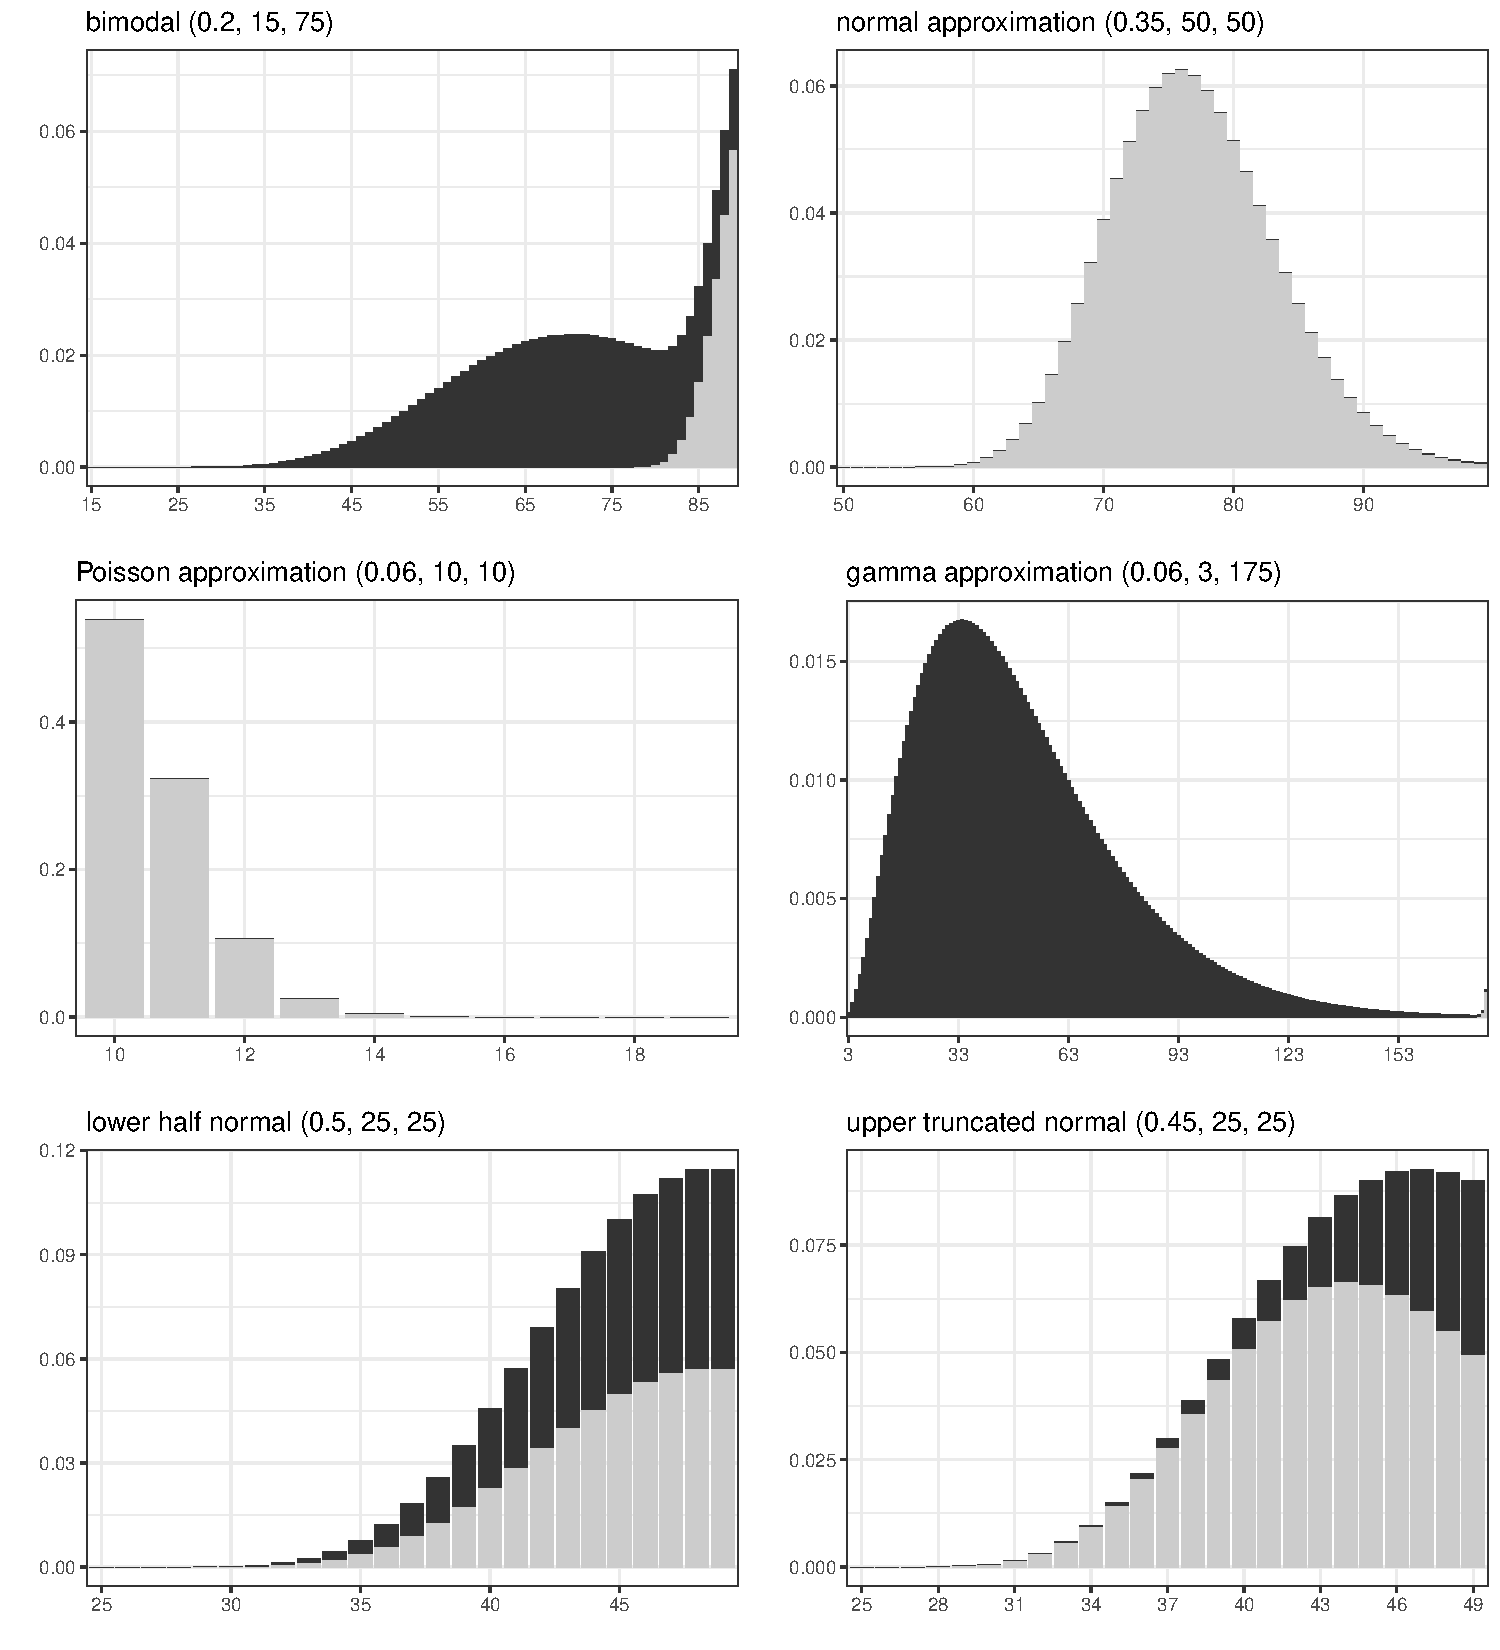
\includegraphics[width=0.8\textwidth]{shapes.pdf}
\end{center}
\caption{Different shapes of the SNB distribution with parameters 
($p$, $s$, $t$), as given. Black areas indicate the mass contributed by reaching
$s$ responders before $t$ non-responders. Grey indicates
mass contributed by reaching $t$ non-responders first. \label{shapes.fig}}
\end{figure}

The SNB is a generalization of the negative 
binomial distribution. When $t$ is large then $Y-s$ has a 
negative binomial distribution with
\begin{equation*}                                    %   (1)   
\mathbb{P}[Y=s+j\ |\ t \text{ is large\ }]        \label{nb1.eq}          
  = {{s+j-1}\choose{s-1}} p^s (1-p)^j
\end{equation*}
for $\,j=0, 1,\ldots\,$. A similar statement can be made when $s$ is large
and $t$ is moderate. As a result, with proper parameter choice, the SNB
can mimic other probability distributions in a manner similar to 
those described in \cite{Peizer1968} and \cite{Best1974}. Examples are
shown in in Fig.~\ref{shapes.fig}. 

The SNB generalizes both the minimum (riff-shuffle) and maximum negative
binomial distributions up to a translation of the support.
For the special case of $\,s=t,$ the distribution of $\,Y\,$ is the
riff-shuffle, or minimum negative binomial 
distribution~\citep{Uppuluri1967,Johnson2005}.
The maximum negative binomial \cite{Johnson2005,Zhang2000,Zelterman2005} is 
the smallest number of outcomes necessary to 
observe at least $s$ responders {\em and} $s$ non-responders. This is equivalent
to a translated version of the riff-shuffle. 

%\section{Connection Between the SNB and the Binomial Tail Probability}

%There is a close connection between the tail probabilities of the SNB and the 
%binomial distributions.
%The probability of reaching the success endpoint in an 
%SNB($p$, $s$, $t$) random variable is 
%equal to the probability of at least $s$ successes in a binomial distributed 
%random variable with size $s+t-1$ and success probability $p$. 
%Likewise, the probability of reaching the failure endpoint is equal
%to the probability of at most $s-1$ successes in a binomial distribution. 
There is also an equivalence between the probability of reaching an endpoint 
in the SNB model and the tail probability of the binomial distribution.
Specifically, the probability that the number of responders is at least 
$s$ in the binomial model is the same as the probability the treatment succeeds 
(reaches $s$) in the SNB model.
\begin{prop} \label{binomial_tail}
Let $Y$ be distributed as SNB($p$, $s$, $t$) and let $X_Y$ correspond
to the number of responders at the end of the trial. Let 
$B$ be distributed binomial with index parameter $n=s+t-1$ and response 
probability $p$. Then
\begin{equation}
\mathbb{P}[B \geq s] = \mathbb{P} [X_Y = s].
\end{equation}
\end{prop}
\begin{proof}
The binomial tail probability is
\begin{equation*}
\mathbb{P}[B \geq s] = 1 - \mathcal{I}_{1-p}(s, t)
\end{equation*}
The corresponding success probability is
\begin{equation} \label{eqn:success}
\mathbb{P} [X_Y = s] 
  = \sum_{k=s}^{s+t-1} {k-1 \choose s-1} p^s (1-p)^{k-s}.
\end{equation}
Let $i=k-s$. Since
\begin{equation*}
{i+s-1 \choose s-1} = {i+s-1 \choose i},
\end{equation*}
the summation in (\ref{eqn:success}) can be rewritten as
\begin{align*}
\mathbb{P} [X_Y = s] &= \sum_{i=0}^{t-1} {i+s-1 \choose i} p^s (1-p)^i\\
  &= 1 - \mathcal{I}_{1-p}(t, s)
\end{align*}
completing the proof.
\end{proof}

To illustrate this result, let us return to our initial example
where $s=7$, $t=11$, and $p=0.2$.  The probability masses in
Fig.~\ref{fig:snb_bin_compare} represented in 
black are equal in panels (a) and (b) as are the masses in grey.
The probability that $s$
responders are reached in the SNB process is the same as the binomial 
probability of at least seven responders. Likewise, the probability that $t$ 
non-responders are reached in the SNB process is the same as the binomial
probability of zero through six responders.

\begin{figure}[t!]
\centering
\subfloat[SNB distribution]{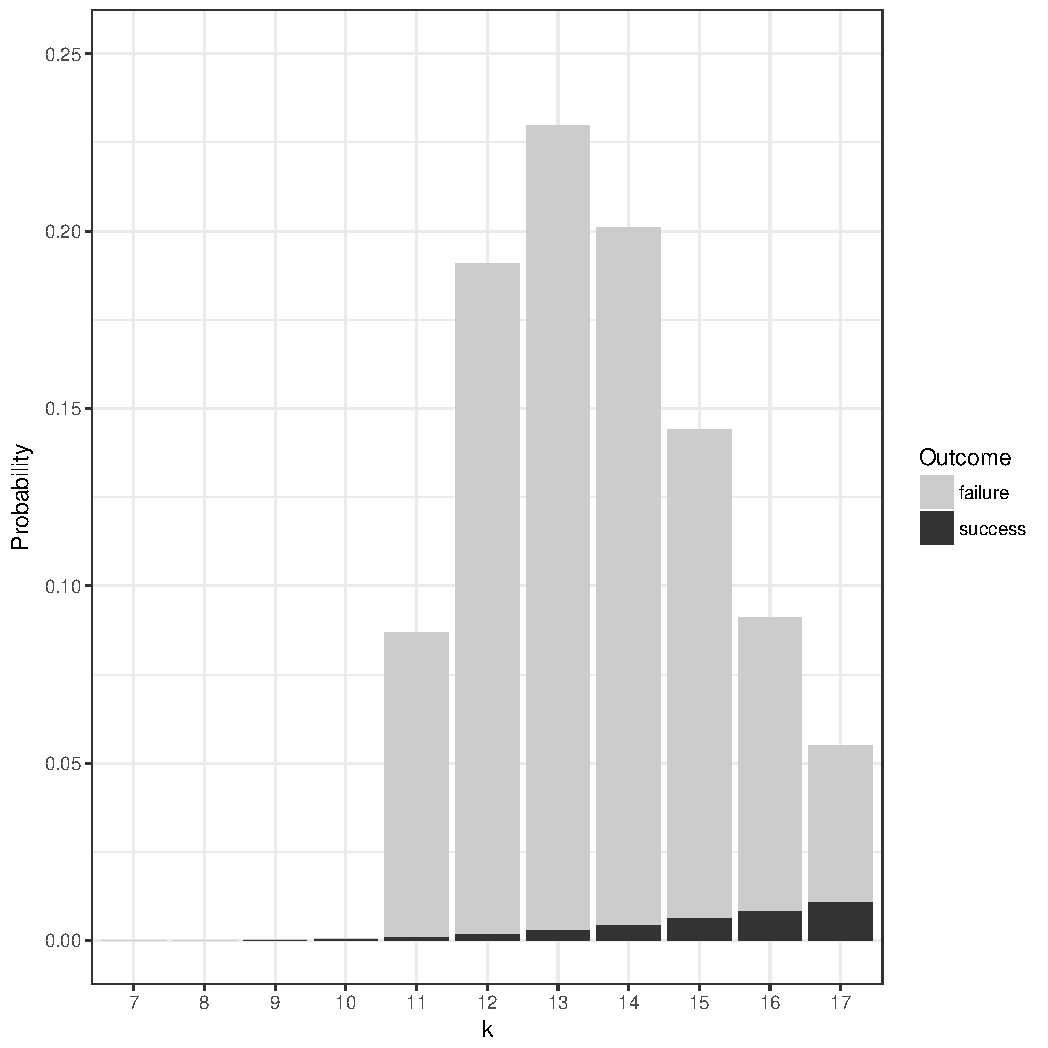
\includegraphics[width=0.5\textwidth]{snb_density.pdf}}
\hfill
\subfloat[binomial distribution]{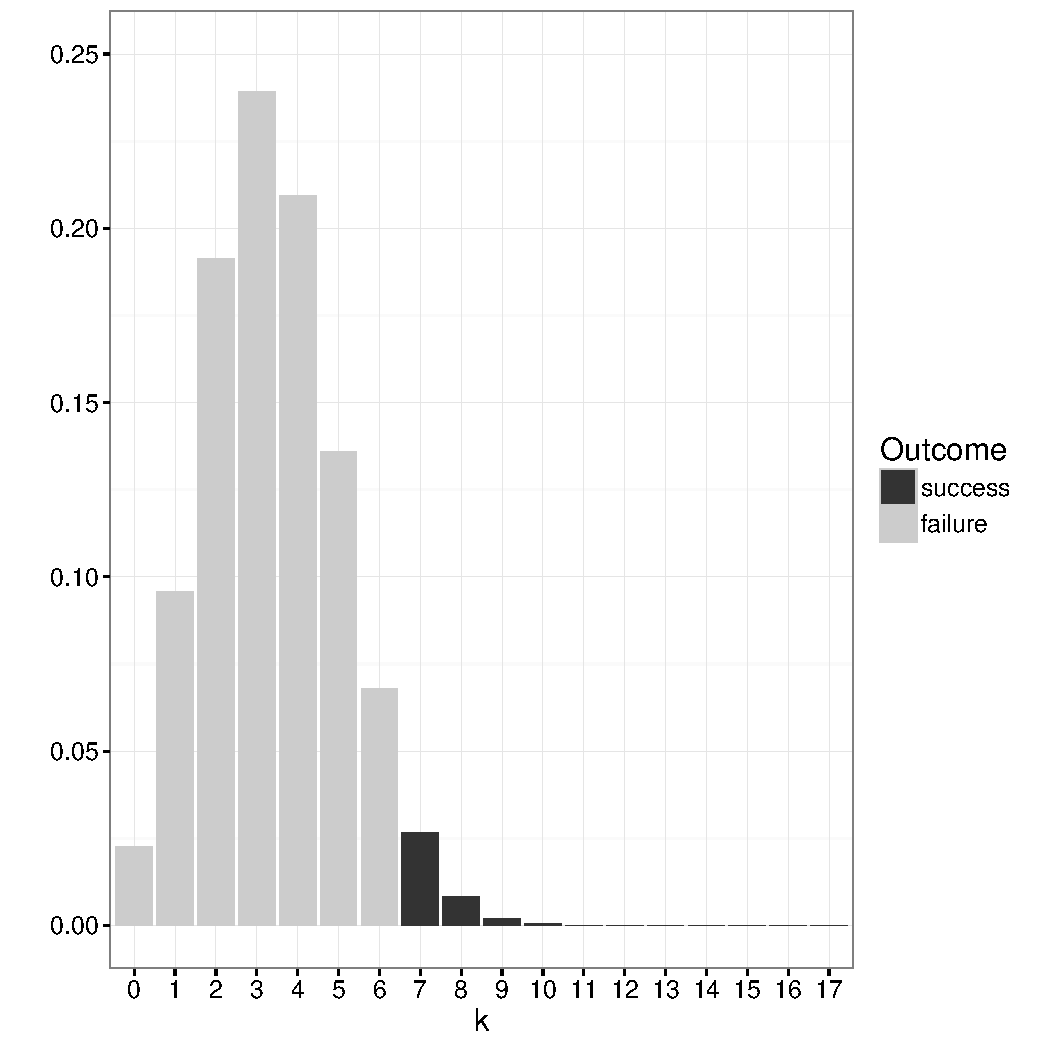
\includegraphics[width=0.5\textwidth]{bin_density.pdf}}
\caption{
SNB(0.2, 7, 11) with mass contributed from 
7 responders (black) or 11 non-responders (grey) along with 
Binomial(0.2, 17) with at least 2 responders (black) or fewer (grey).
}
\label{fig:snb_bin_compare}
\end{figure}

\section{The Moment Generating Function}

The moment generating function for the SNB is calculated in a manner similar to 
that of two negative binomial distributions. 
\begin{prop} Let $Y$ be distributed SNB with parameters $p$, $s$, and $t$.
Then the moment generating function (MGF) of $Y$ is
\begin{equation} \label{eqn:mgf}
\mathbb{E}~e^{xY} = \left(\frac{p e^x}{1 - qe^x}\right)^s 
  \mathcal{I}_{1-qe^x} (s, t) + \left(\frac{qe^x}{1-pe^x}\right)^t 
  \mathcal{I}_{1-pe^x}(t, s)
\end{equation}
for $q = 1-p$ and is defined for 
$x < \min \left\{\log(1/p), \log(1/q) \right\}$.
\end{prop}
\begin{proof}
The MGF of the SNB is:
\begin{equation*}
\mathbb{E}~e^{xY} = \sum_{k=s}^{s+t-1} {k-1 \choose s-1} p^s q^{k-s} e^{kx} 
  + \sum_{k=t}^{s+t-1} {k-1 \choose t-1} p^{k-t} q^t e^{kx}
\end{equation*}
and can be rewritten as:
\begin{equation} \label{eqn:first_sum}
\mathbb{E}~e^{xY} = \sum_{k=s}^{s+t-1}{k-1 \choose s-1} (pe^x)^{s} (qe^x)^{k-s} 
  + \sum_{k=t}^{s+t-1}{k-1 \choose t-1} (qe^x)^t (pe^x)^{k-t}.
\end{equation}
The first summation in (\ref{eqn:first_sum}) satisfies
\begin{align*}
\sum_{k=s}^{s+t-1}{k-1 \choose s-1} (pe)^{sx} (qe^x)^{k-s} &= 
  \left(\frac{pe^x}{1 - qe^x}\right)^s \ \ \sum_{k=s}^{s+t-1} {k-1 \choose s-1} 
    (qe^x)^{k-s} (1-qe^x)^s \\
  &= \left(\frac{pe^x}{1 - qe^x}\right)^s \mathcal{I}_{1-qe^x}(s, t).
\end{align*}
Since the $p$ parameter in $\mathcal{I}_p$ has support on zero 
to one, we have $0 \leq pe^x < 1$. This implies $x < -\log(p)$.
A similar expression can be derived for the second summation in 
(\ref{eqn:first_sum}) and results in
the constraint $x < -\log(1-p)$.
\end{proof}

Depending on the parameter values the SNB can be approximated by 
the geometric, normal, gamma, and Poisson
distributions.

\begin{prop}
The MGF of the SNB converges to that of the negative binomial when either
$s$ or $t$ gets large. That is
\begin{equation*}
lim_{t\to\infty} \ \mathbb{E} e^{xY} = \left( \frac{pe^x}{1-qe^x} \right)^s
\end{equation*}
as. The analogous result holds when $s \rightarrow \infty$.
\end{prop}
\begin{proof}
The second incomplete beta function in (\ref{eqn:mgf}) can be written
in terms of a cumulative binomial distribution
\begin{equation*}
\mathcal{I}_{1-pe^x}(t, s) = \mathbb{P}\left[ B \leq s-1 \right]
\end{equation*}
where $B$ is distributed as
Binomial($t-k$, $pe^x$). From Chebychev's inequality %\cite{Hoeffding1963}
it follows that
\begin{equation} \label{eqn:hoeffding}
\mathbb{P}\left[ B \leq s-1 \right] \leq 
  \frac{ (t-k) pe^x (1-pe^x) }{ \left(s - (t-k)pe^x\right)^2 }
\end{equation}
As $t$ gets large $\mathcal{I}_{1-pe^x}(t, s)$ tends to zero
and $\mathcal{I}_{1-qe^x}(s, t)$ approaches 
one. The proof follows by realizing 
\begin{equation*}
0 < \frac{qe^x}{1-pe^x} < 1
\end{equation*}
over the support of $x$.
\end{proof}

When $s=1$ and $t$ is large the SNB's MGF is approximately 
the same as that of the
geometric distribution. The negative
binomial can therefore be seen as a sum of i.i.d. geometric distributions.
For an appropriately large number of distributions, the central limit theorem
yields a normal approximation.

Drawing connections to the gamma and Poisson distributions can also be shown.
A connection to the gamma distribution well-studied problem in the 
literature (see \cite{Best1974,Ord1968,Guenther1972} for examples). 
A connection to the Poisson appears in \cite{Anscombe1950} where
it is shown that when the mean of a Poisson is proportional
to a chi-square distribution with $2k$ degrees of freedom
then the negative binomial is obtained. 
Both of these approximations work by equating cumulants and then showing 
that differences between the cumulant generating
functions converge to zero.

The lower-half normal distribution can be approximated by setting $s=t$
for appropriately large $s$ and $t$ and $p = 0.5$. In this
case, the SNB can be viewed as identical, negative binomial distributions
approximating a normal and truncated at the median.

\section{The Posterior and Predictive Probability Distribution}

Let us consider the Bayesian setting where the rate parameter is distributed 
as Beta($\alpha$, $\beta$) and denoted $P$.
The posterior distribution of $P$ is proportional to the 
likelihood, given by the function
%f_P(p, \alpha, \beta ) f_{Y|P}(p, k, s, t) &= 
\begin{align} \label{eqn:ptl}
f_{P|Y}(p, k, s, t, & \alpha, \beta) \propto
  \frac{ {k-1 \choose s-1} }{B(\alpha, \beta)} p^{\alpha +s -1} 
    (1-p)^{k+\beta-s-1} \\
  & + \frac{ {k-1 \choose t-1} }{B(\alpha, \beta)} p^{k+\alpha -t -1} 
    (1-p)^{\beta+t-1} \nonumber
\end{align}
where $0 \leq p \leq 1$, $s \leq k \leq s+k-1$, and $t \leq k \leq s+k-1$.

The predictive distribution of the SNB can be found as by integrating
$p$ over the interval zero to one and applying the definition of the 
beta function.
\begin{align} \label{eqn:predictive}
f_{Y}(&k, s, t, \alpha, \beta) = 
  \int_0^1 f_P(p | \alpha, \beta )  f_{Y|P}(p, k, s, t) dp \nonumber \\ 
 & = {k-1 \choose s-1} \frac{B\left(\alpha+s, k-s+\beta \right)}{B(\alpha, \beta)} 
    + {k-1 \choose t-1} 
    \frac{B\left(\alpha + k - t, t+\beta\right)}{B(\alpha, \beta)}.
\end{align}
If both $\alpha$ and $\beta$ are non-negative integers then the predictive
distribution is a mixture of hypergeometric distributions. 
\begin{align*} \label{eqn:hypergeo}
f_{Y}(k, s, t, \alpha, \beta) = 
  \frac{ {k - 1 \choose s - 1 } 
         {\alpha + \beta \choose \alpha} }{
         {\alpha + \beta + k - 1 \choose \alpha + s}}
  \frac{\alpha}{\alpha + \beta}
  \frac{ \beta }{ k-s+\beta } +
  \frac{ {k - 1 \choose t - 1} 
         {\alpha + \beta \choose \beta} 
         }{
         {\alpha + \beta + k -1 \choose t + \beta}
       }
  \frac{ \beta }{ \alpha + \beta}
  \frac{ \alpha }{ k-t + \alpha}
\end{align*}
The ratio of combinations in the first term can be interpreted as the
probability of $s-1$ responders from $k-1$ patients in $\alpha + s$ draws
from a population size of $\alpha + \beta + k - 1$. This value is multiplied
by $\alpha / (\alpha + \beta)$, the expected response rate of the prior. 
The final term in the product weigths the prior based on the number
of non-responders ($k-s$). Terms in the second summand are interpreted similarly
for non-responders.

The ratio of (\ref{eqn:ptl}) divided by (\ref{eqn:predictive}) gives the 
posterior distribution of $P$. It is a mixture of beta distributions. The
mixing parameter depend on the endpoints ($s$ and $t$), the number of enrollees needed to reach an endpoint ($k$), and the prior parameters ($\alpha$ and
$\beta$).

\begin{figure}[t!]
\centering
\includegraphics[width=\textwidth]{beta-mixture.pdf}
\caption{
The posterior distribution of the response probability with 
the Jeffreys prior ($\alpha=\beta=1/2$) for the trial where
$s=7$, $t=11$, $k=15$.
}
\label{fig:beta_mixture}
\end{figure}

The posterior result above is for the case where the parameters are known
and the endpoint is not. That is, we do not which boundary was reached.
Fig.~\ref{fig:beta_mixture} shows this distribution based on the 
parameters in the hypothetical trial assuming the
Jeffreys prior \citep{Jeffreys1946}.  If we include the fact that the
trajectory reaches the endpoint then the second terms in (\ref{eqn:ptl}) and
(\ref{eqn:predictive}) are both zero and the posterior distribution is
Beta(7.5, 8.5). This is proportional to the area labeled ``success'' in 
Fig.~\ref{fig:beta_mixture}.

\section{Powering Trials using Confidence Sets}

The previous section shows the posterior distribution $P$ at each of the 
endpoints in the domain is defined by a Beta distribution. This fact can be 
used to provide power calculations based on confidence sets with specified 
minimum response rate. Let $\mathcal{P}_s(s,t)$ be the set of random variables
associated success. Then a trial whose minimum
response rate is $p_{min}$ at a significance level of at least $\alpha_C$ is 
one where each distribution is at least $p_{min}$ with probability 
$1-\alpha_C$.  That is,
\begin{equation} \label{pwr_signif}
  \mathbb{P} \left[X > p_{min} \right] > (1 - \alpha_C) 
  \ \ \forall X \in \mathcal{P}_s(s,t)
\end{equation}
Letting $\mathcal{Q}_t(s,t)$ be the set of random variables associated with
failure, a trial whose power is at least $1-\beta_C$ has
\begin{equation*} \label{pwr}
  \mathbb{P} \left[X < p_{min} \right] < \beta_C
  \ \ \forall X \in \mathcal{Q}_t(s,t).
\end{equation*}

\begin{prop} \label{alpha_c}
Let $P_k$ be the posterior distribution of reaching the success endpoint
at the $k$th enrollment with density
\begin{equation*}
f_k(p) = \frac{ {k-1 \choose s-1} }{B(\alpha, \beta)} p^{\alpha +s -1} 
    (1-p)^{k+\beta-s-1}.
\end{equation*}
If $0 \leq \alpha_C \leq 1 - 1/k$ then 
\begin{equation}
\mathbb{P} \left[P_k \geq \alpha_C \right]  \leq
  \mathbb{P} \left[P_{k-1} \geq \alpha_C \right].
\end{equation}
\end{prop}
\begin{proof}
Consider the ratio of the posterior distributions
\begin{align*}
\frac{f_k(p)}{f_{k+1}(p)} &= 
  \frac{\frac{ {k-1 \choose s-1} }{B(\alpha, \beta)} p^{\alpha +s -1} 
    (1-p)^{k+\beta-s-1}}
    {\frac{ {k \choose s-1} }{B(\alpha, \beta)} p^{\alpha +s -1} 
    (1-p)^{k+\beta-s}} \\
  &= \frac{ p^{\alpha +s -1} (1-p)^{k+\beta-s-1} }
    {k p^{\alpha +s -1} (1-p)^{k+\beta-s}} \\
  &= \frac{1}{k(1-p)}.
\end{align*}
This implies that the density $f_{k+1}(p)$ is greater than $f_k(p)$ for
all values of $0 \leq p \leq 1 - 1/k$. This implies the
integral of $f_{k+1}(p)$ must also be greater than $f_k(p)$ over a similar
interval. The result follows by realizing that this relationship is reversed
over the complement of the interval.
\end{proof}

The maximum significance of a trial is 
$\mathbb{P} \left[P_{s+t-1} \leq \alpha_C \right]$ Proposition \ref{alpha_c}
guarantees the significance for all other success endpoints will be smaller.
A similar calculation can be performed for power to show that the minimum
power is $\mathbb{P} \left[Q_{s+t-1} \leq 1 - \beta_C \right]$ where
$Q_{s+t-1}$ is the posterior distribution of reaching a trial failure
at the $s+t-1$ step.

These two results imply a relatively simple procedure for finding the sample
size for trials of this type. A minimum response rate, maximum significance,
and minimum power are selected. The task is to find the values of $s$ and
$t$ that fulfill these requirements given the minimum response. Start with 
$s = t = 1$. If the maximum significance criterion is not met then increase
$s$ by one. If the minimum power criterion is not met then increase $t$ by
one. Repeat the procedure until both criteria have been met. The sample
size is then determined by the calculation $s+t-1$.

\section{A Bayesian Sequential Probability Ratio Test}

Keeping $s$ and $t$ constant for all time steps in the trial provides 
mathematical convenience since the distribution can be calculated in closed 
form. It should be noted though that any set of endpoints where every endpoint 
can be reached defines a valid probability distribution. This fact allows us 
to define new stopping criteria when defining success and failure endpoints.

One such set of stopping criteria is based on the confidence sets of the 
response rate from the previous section. Proposition (\ref{alpha_c}) shows 
$\mathbb{P_k} [P_k \geq \alpha_c] \leq \mathbb{P}[P_{k-1} \geq \alpha_c]$. 
That is, the probability the response rate is at least $p_{min}$ is increasing 
in $-k$. This observation implies we can guarantee that the response rate is 
greater than $p_min$ before reaching $s$ when a greater proportion of 
successful outcomes are observed.

Therefore, we can define a new set of success and failure endpoints that stop 
a trial as soon as the response distribution is at least $\alpha_c$ or the 
criteria cannot be met, based on the sample size. This design is analogous to 
the Sequential Probability Ratio Test (SPRT) \cite{Wald1945} in that the 
stopping criteria is defined by the ratio responders to non-responders, 
through the beta prior. It has two distinct advantages though. First, unlike 
the SPRT it has a maximum sample size, similar to the MaxSPRT 
\cite{Kulldorff2011}, making it appropriate for small-sample studies. Second, 
the stopping criteria are based on both a minimum response rate as well as the 
degree of certainty, $1-\alpha$, that this response rate has been attained.




\section{The Approximate Distribution for Two Linear Boundaries}

Consider an alternative visualization of the sample path counting the 
number of responders and non-responders in the vertical and horizontal 
direction respectively, as in Figure \ref{fig:zplot}. This alternative
formulation can be rotated and scaled to form a random walk on the integers.
A functional central limit can be then applied when the endpoints are 
sufficiently far from the origin and the process converges to a Brownian 
motion. The hitting time of the success and failure endpoints is under 
this reparameterization is a mixture of normal distributions.

\begin{figure}[t!]
\centering
\includegraphics[width=\textwidth]{zplot.pdf}
\caption{
An alternative visualization of the hypothetical trial.
}
\label{fig:zplot}
\end{figure}

For a response rate $p$, the expected direction of each step in the sample 
path is $\tan^{-1}(p)$ radians from the vertical direction.
If the graph is rotated $\pi/2- \Theta$ radians then the 
expected value of the process is zero at any time.
Let $\Theta = tan^{-1}(p)$. Then, after rotation, the process moves 
$\sin \Theta$ units in the horizontal direction and $\cos \Theta$ units in 
the positive vertical direction for each response. Each non-response 
corresponds to $\cos (\Theta)$ units in the horizontal direction and 
$\sin \Theta$ units in the negative vertical direction. The rotation is shown 
pictorially in Figure \ref{fig:theta_rot}.

\begin{figure}[bp!] 
\centering
\subfloat[Before rotation]{\includegraphics[width=0.45\textwidth]{proc.pdf}}
\hfill
\subfloat[After rotation]{\includegraphics[width=0.45\textwidth]{proc-rot.pdf}}
\caption{
The direction of a single step in the binomial process before (a) and after
rotation (b).
}
\label{fig:theta_rot}
\end{figure}

After the rotation, a response step is normalized by $\sin(\pi/2-\Theta)$ in the
vertical direction and $\cos(\pi/2 - \Theta)$ in the horizontal direction.
Likewise, a non-response step is normalized by $\sin(\Theta)$ and
$\cos(\Theta)$ in the vertical and horizontal direction respectively. Each
step is a Rademacher random variable. The
resulting process forms a random walk on the integers. Let $m$ be the
shortest path from the origin to any endpoint, let step $k=mt$
the process, and let $R_i$ be a sample from a Rademacher random variable. Then
it is well known that a c\'{a}dl\'{a}g version of the rescaled process on the
natural filtration converges to a Brownian motion as $m$ gets large
\begin{equation*}
t \frac{1}{\sqrt{t m}} \sum_{i=0}^{t m} R_i \rightarrow
B(t).
\end{equation*}

The density of the first time a Brownian motion hits a sloping line with
intercept $a$ and is \cite{Bachelier1900}
\begin{equation}
f_{a,b}(t) = \frac{a}{t^{3/2}} \phi \left(\frac{a + bt}{\sqrt{t}} \right)
\end{equation}
where $\phi(t)$ is the density of the standard normal distribution at $t$.
Therefore, for success and failure endpoints defined by lines 
$a + bt$ and $a' + b't$ with support $[s_0 \leq t \leq s_m]$ and 
$[r_0 \leq t \leq r_m]$ respectively, the density of the SNB approximation
is 
\begin{equation}
f(t) = \frac{ f_{a,b}(t)[s_0 \leq t \leq s_m] + 
  f_{a',b'}(t)[r_0 \leq t \leq r_m]}{
  \int_{s_0}^{s_m} f_{a,b}(x) dx + \int_{r_0}^{r_m} f_{a',b'}(x) dx}.
\end{equation}



\bibliography{mybibfile}

\end{document}
